%% HKUST unofficial poster template
% By Ching Ting Leung, class of 2025 in BEng

% Forked from Gemini theme
% https://github.com/anishathalye/gemini

% Required Compiler: LuaLaTeX

\documentclass[final]{beamer}

% ====================
% Packages
% ====================

\usepackage[T1]{fontenc}
\usepackage{lmodern}
\usepackage[size=custom,width=120,height=72,scale=1.0]{beamerposter} % default
% \usepackage[orientation=landscape,size=a0,scale=1.4]{beamerposter} % custom
% scale: scaling factor of all font

\usetheme{gemini}
\usecolortheme{Tuebingen} % Customize in beamercolorthemeTuebingen.sty

\usepackage{graphicx}
\usepackage{booktabs}
\usepackage{tikz}
\usepackage{pgfplots}
\pgfplotsset{compat=1.14}
\usepackage{anyfontsize}

\usepackage{url}

% ====================
% Lengths
% ====================

% If you have N columns, choose \sepwidth and \colwidth such that
% (N+1)*\sepwidth + N*\colwidth = \paperwidth
\newlength{\sepwidth}
\newlength{\colwidth}
\setlength{\sepwidth}{0.02\paperwidth}
\setlength{\colwidth}{0.225\paperwidth}

\newcommand{\separatorcolumn}{\begin{column}{\sepwidth}\end{column}}

% ====================
% Title
% ====================

\title{Current State of Language Technologies in Sorbian Languages}

\author{Daniel Sobe \inst{1} \and Ivan Kraljevski \inst{2}}

\institute[shortinst]{\inst{1} Załožba za serbski lud, Budyšin / Foundation for the Sorbian people, Bautzen, Germany \and \inst{2} Fraunhofer Institute for Ceramic Technologies and Systems IKTS, Dresden, Germany}

% ====================
% Footer (optional)
% ====================

\footercontent{
  \href{https://zalozba.de}{https://zalozba.de} \hfill
  LT4All 2025, Paris \hfill
  \href{mailto:d.zoba@zalozba.de}{d.zoba@zalozba.de}}
% (can be left out to remove footer)

% ====================
% Logo (optional)
% ====================

% use this to include logos on the left and/or right side of the header:
\logoright{
\includegraphics[height=7cm]{SfdsV_Logo2015_CMYK.jpg}}
\logoleft{
\includegraphics[height=7cm]{FHG_Logo.png}}

% ====================
% Body
% ====================

\begin{document}

\begin{frame}[t]
\begin{columns}[t]
\separatorcolumn

\begin{column}{\colwidth}

  \begin{block}{Speech recognition (HSB)}

    \heading{Traditional approach}

    recITKS (proprietary) - optionally Kaldi
        
    \heading{AI approach}

    Huggingface whisper

    \heading{Applications}

    Youtube subtitles/translations (working)

    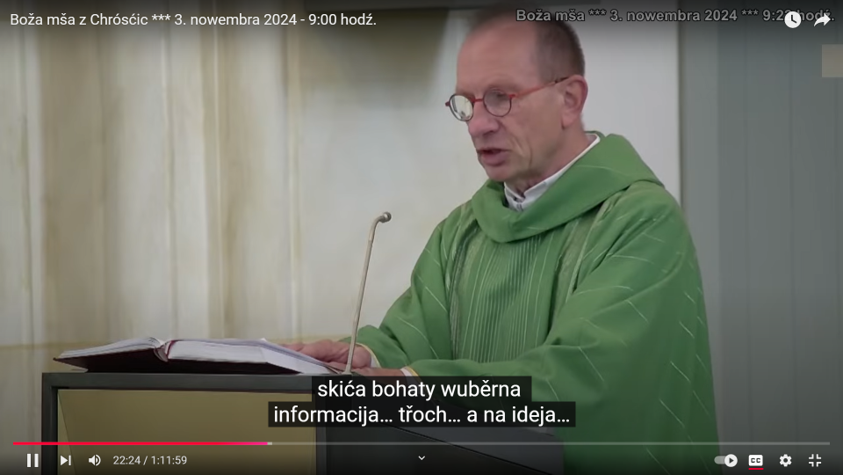
\includegraphics[width=\colwidth]{citanje.png}

    Subtitles/translations in web conferences (Jitsi, in progress)
    
    Offline transcriptions (working)
    
  \end{block}

  \begin{block}{Simultaneous translation (HSB)}

    combination of recognition and translation

    \begin{figure}
        \centering
        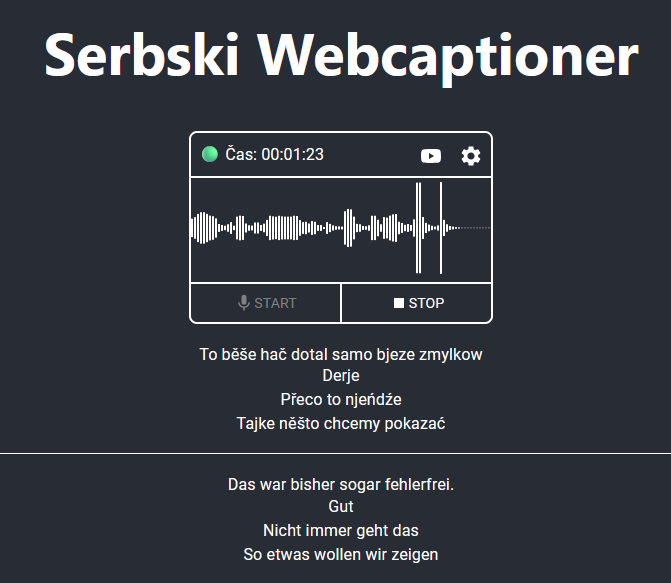
\includegraphics[width=0.8\colwidth]{webcaptioner_klein.png}
        \label{fig:webcaptioner}
    \end{figure}

  \end{block}

\end{column}

\separatorcolumn

\begin{column}{\colwidth}

  \begin{block}{Machine translation (HSB/DSB)}

    sotra project

    \begin{itemize}
      \item \textbf{needed} corpus management
      \item \textbf{provided technology} Fairseq
    \end{itemize}

    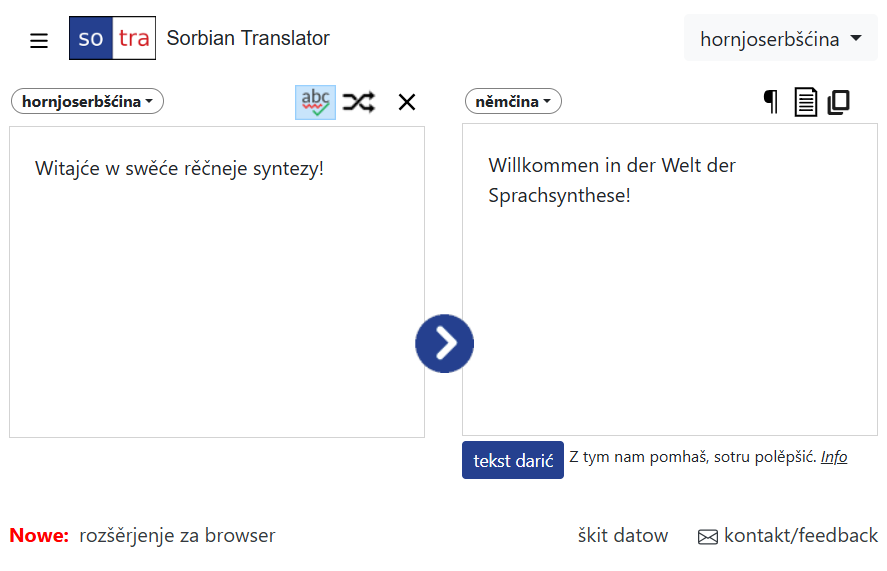
\includegraphics[width=\colwidth]{sotra.png}

  \end{block}

  \begin{block}{Language research (HSB/DSB)}  
  
    \heading{sorbian institute}

    hornjoserbsce.de

    dolnoserbski.de

    \begin{figure}
        \centering
        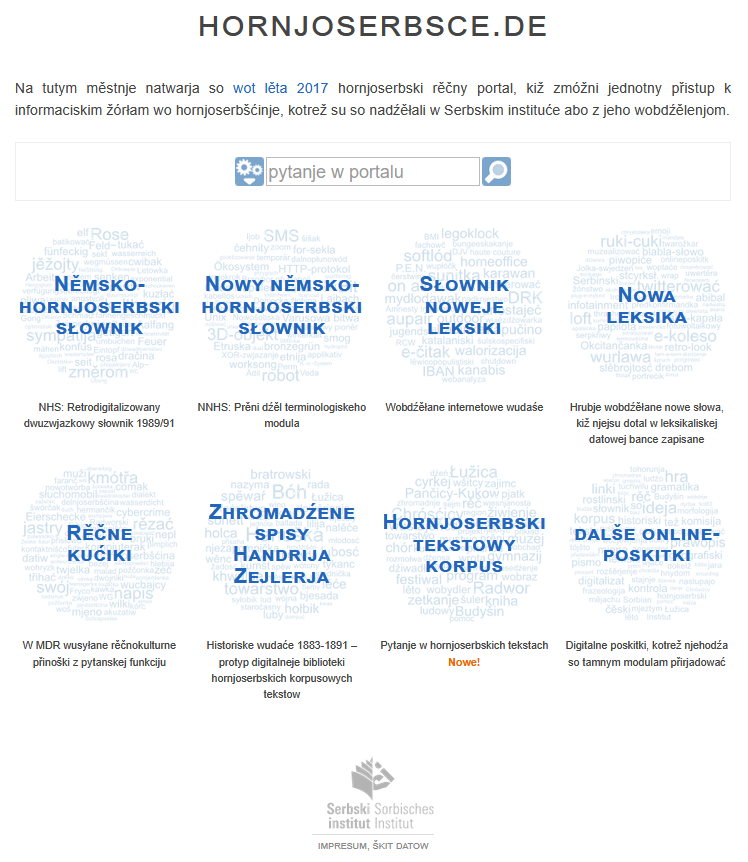
\includegraphics[width=0.7\colwidth]{hornjoserbsce_gross.png}
        \label{fig:hornjoserbsce}
    \end{figure}

  \end{block}

\end{column}

\separatorcolumn

\begin{column}{\colwidth}

  \begin{block}{Language learning (HSB)}

    \heading{soblex}
    
    soblex project\cite{soblex}

    dictionary

    \begin{figure}
        \centering
        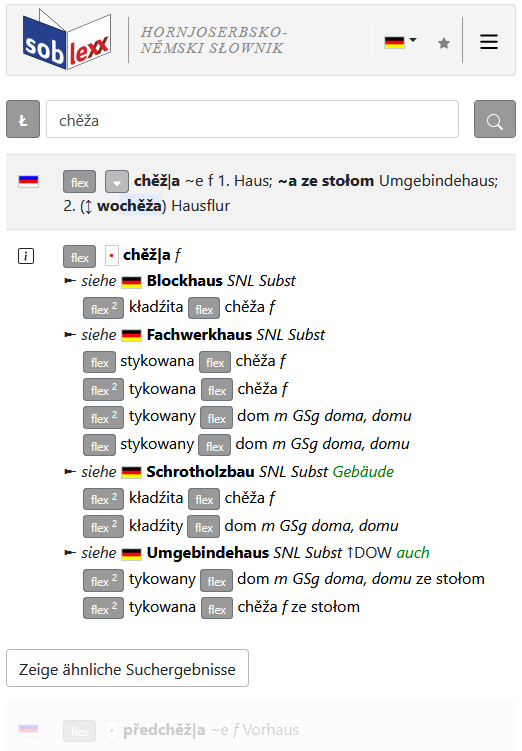
\includegraphics[width=0.7\colwidth]{soblex_suche.png}
        \label{fig:soblexsearch}
    \end{figure}

    flexions

    \begin{figure}
        \centering
        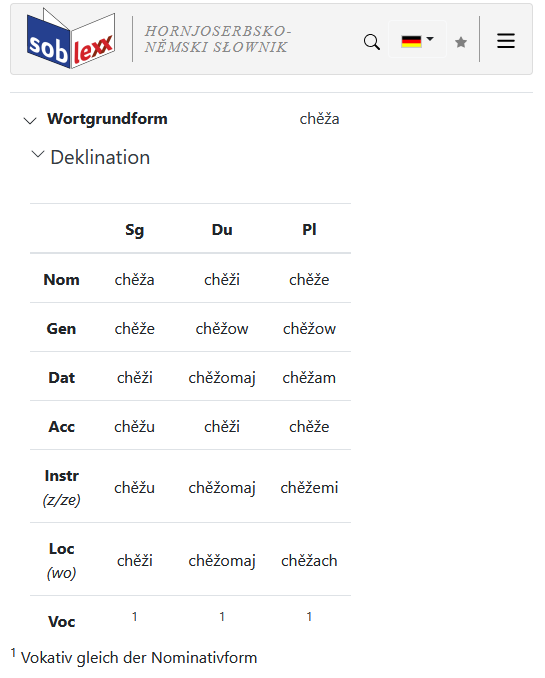
\includegraphics[width=0.7\colwidth]{soblex_klein.png}
        \label{fig:soblex}
    \end{figure}

  \end{block}

\end{column}

\separatorcolumn

\begin{column}{\colwidth}

  \begin{block}{Speech synthesis}

    \heading{Traditional approach (HSB/DSB)}

    MaryTTS

    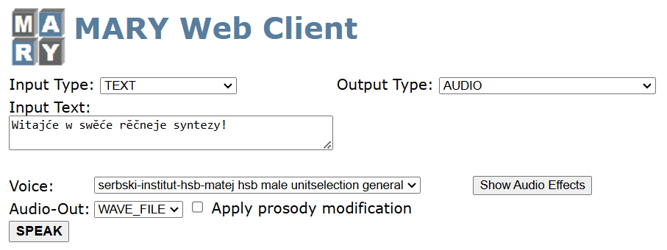
\includegraphics[width=\colwidth]{marytts_small.png}

    \heading{AI approach (HSB)}

    Coqui TTS (bamborak\cite{bamborak})

    \begin{figure}
        \centering
        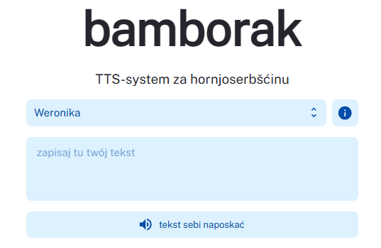
\includegraphics[width=0.75\colwidth]{bamborak_small.png}
        \label{fig:bamborak}
    \end{figure}
    

  \end{block}
  
  \begin{block}{References}

%    \nocite{*}
    \footnotesize{\bibliographystyle{plain}\bibliography{poster}}

  \end{block}

\end{column}

\separatorcolumn
\end{columns}
\end{frame}

\end{document}
